%============================================================
% HYPOTHESES
%============================================================

\section{Hypotheses}

%------------------------------------------------------------
% HYPOTHESIS - SLIDE 1
%------------------------------------------------------------

\begin{frame}
    \frametitle{Hypothesis 1: Effect of Attention Modulation}

    \small

    \begin{block}{Hypothesis 1}
        Nếu hệ số $d$ điều khiển mức độ đóng góp của retrieved
        passages, thì LM loss sẽ thay đổi theo $d$.
    \end{block}

    \vspace{0.3cm}

    \begin{center}
    \[
        A =
        dA_{\mathrm{doc}}
        +
        (1-d)A_{\mathrm{no\_doc}}
    \]

    \vspace{0.15cm}

    \[
        d \uparrow
        \quad\Longrightarrow\quad
        \text{retrieved information đóng góp nhiều hơn}
    \]
    \end{center}

    \vspace{0.25cm}

    \begin{block}{Expected}
        \centering
        Mức độ thay đổi của $L_{LM}(d)$ phụ thuộc vào
        \textbf{độ hữu ích của retrieved passages}.
    \end{block}

\end{frame}


%------------------------------------------------------------
% HYPOTHESIS - SLIDE 2
%------------------------------------------------------------

\begin{frame}
    \frametitle{Hypothesis 2: Gradient as a Learning Signal}

    \small

    \begin{block}{Hypothesis 2}
        Nếu $d$ ảnh hưởng đến LM loss, gradient
        $\frac{\partial L_{LM}}{\partial d}$ có thể cung cấp
        tín hiệu cho retrieval decision.
    \end{block}

    \vspace{0.3cm}

    \begin{center}
    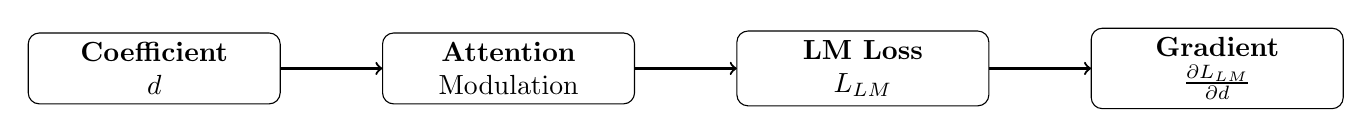
\begin{tikzpicture}[
        every node/.style={align=center},
        box/.style={
            draw,
            rounded corners,
            minimum width=3.2cm,
            minimum height=0.85cm
        },
        arrow/.style={
            ->,
            thick
        }
    ]

        \node[box] at (0,0)
        {\textbf{Coefficient}\\
        $d$};

        \node[box] at (4.5,0)
        {\textbf{Attention}\\
        Modulation};

        \node[box] at (9,0)
        {\textbf{LM Loss}\\
        $L_{LM}$};

        \node[box] at (13.5,0)
        {\textbf{Gradient}\\
        $\frac{\partial L_{LM}}{\partial d}$};

        \draw[arrow] (1.6,0) -- (2.9,0);
        \draw[arrow] (6.1,0) -- (7.4,0);
        \draw[arrow] (10.6,0) -- (11.9,0);

    \end{tikzpicture}
    \end{center}

    \vspace{0.3cm}

    \begin{itemize}
        \item Retrieved information hữu ích
        $\rightarrow$ tăng $d$ có xu hướng giảm $L_{LM}$.

        \item Retrieved information không hữu ích
        $\rightarrow$ tăng $d$ có xu hướng làm tăng $L_{LM}$.

        \item Do đó, gradient có thể cung cấp
        \textbf{local learning signal}.
    \end{itemize}

\end{frame}


%------------------------------------------------------------
% HYPOTHESIS - SLIDE 3
%------------------------------------------------------------

\begin{frame}
    \frametitle{From Hypotheses to Adaptive Retrieval Timing}

    \small

    \begin{center}
    \begin{tikzpicture}[
        every node/.style={align=center},
        box/.style={
            draw,
            rounded corners,
            minimum width=3.5cm,
            minimum height=0.9cm
        },
        arrow/.style={
            ->,
            very thick
        }
    ]

        \node[box] at (0,0)
        {\textbf{H1}\\
        $L_{LM}(d)$ thay đổi theo $d$};

        \node[box] at (5,0)
        {\textbf{H2}\\
        $\frac{\partial L_{LM}}{\partial d}$};

        \node[box] at (10,0)
        {\textbf{Retrieval Decision}\\
        Learn when to retrieve};

        \draw[arrow] (1.8,0) -- (3.2,0);
        \draw[arrow] (6.8,0) -- (8.2,0);

    \end{tikzpicture}
    \end{center}

    \vspace{0.4cm}

    \begin{block}{Core Hypothesis}
        \centering
        Generation objective có thể cung cấp tín hiệu để học
        \textbf{khi nào cần retrieval}.
    \end{block}

    \vspace{0.3cm}

    \begin{center}
        \[
            \boxed{
            \text{Retrieval usefulness}
            \rightarrow
            L_{LM}(d)
            \rightarrow
            \frac{\partial L_{LM}}{\partial d}
            }
        \]
    \end{center}

    \vspace{0.25cm}

    \begin{block}{Goal}
        \centering
        Học retrieval timing mà không cần
        \textbf{direct decision supervision} hoặc
        \textbf{reinforcement learning}.
    \end{block}

\end{frame}